\newpage
\section{Literature Review}
\setresponsible{Regen Wijaya}
\subsection{Biochar}

Biochar is defined as a carbon-rich pyrogenous, solid product produced from biomass-derived digestate or from biomass itself, which is organic matter, mainly plant or animal waste. Biochar is produced through pyrolysis, which is a thermochemical process under high temperature in an oxygen-limited environment. Unlike charcoal, it is not only used as a renewable fuel but predominantly serves to improve soil fertility, maintain carbon neutrality, and mitigate particular environmental pollution. \cite{Qi2024}    

\subsubsection{Properties of Biochar}
The properties of biochar can be broadly classified into physicochemical characteristics, which together determine its behavior and potential use in soil and environmental applications. Biochar properties vary widely depending on the feedstock material and type of pyrolysis process.

\label{Properties of Biochar}
\subsubsection*{Composition and Content}

Biochar is composed of an organic fraction, including fixed-carbon and volatile matter, as well as an inorganic fraction such as ash. Fixed-carbon component is a solid material that has higher stability at varying thermal conditions, while volatile matter component is easily decomposed at higher temperatures \cite{Wood2024BiocharMolecularData}. 
The higher the fixed-carbon content, the higher its heating value and energy content \cite{Tuominen2025BiocharEnergyBalance}. The organic fraction consists primarily of carbon with small amount of other element, including hydrogen, oxygen, sulfur, nitrogen and phosphorus \cite{Wood2024BiocharMolecularData}. On the other hand, inorganic fraction is made of ash, which contains various mineral components, including Na, Mg, K, Ca, P, and other mineral elements \cite{Sajjadi2019}.

\begin{figure}[ht!]
    \centering
    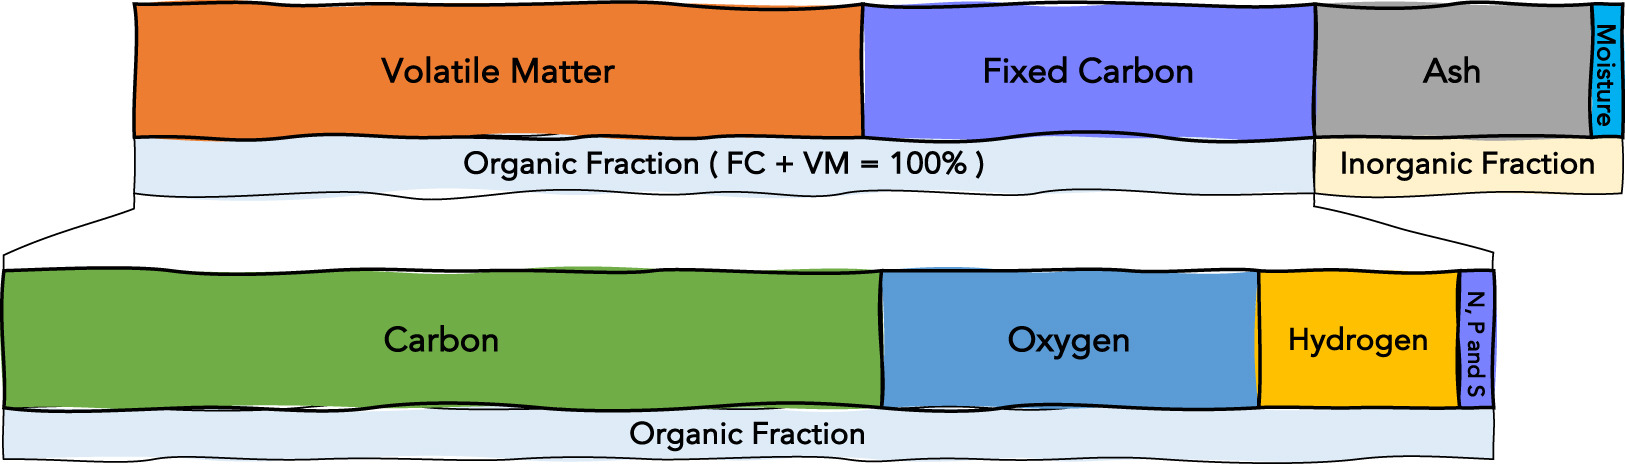
\includegraphics[width=0.8\linewidth]{Abbildungen/gr3_lrg.jpg}
    \caption{Scheme to the chemical composition of biochars.}
    \label{fig:2.1.1.1}
\end{figure}

\begin{table}[H]
\centering
\caption{Elemental composition of biochar. \cite{Sajjadi2019}}
\label{tab:Elemental composition of biochar}

\small
\begin{tabular}{l c c}
\toprule
\textbf{Element} & \textbf{Symbol} & \textbf{Typical content (\%)} \\
\midrule
Carbon   & C & 40--70 \\
Oxygen   & O & 10--45 \\
Hydrogen & H & 1--5 \\
Nitrogen & N & 0--3 \\
Sulfur   & S & $<$1 \\
\bottomrule
\end{tabular}
\end{table}

\newpage
The content of biochar is significantly influenced by the bulk composition of the feedstock. Wood and crop-derived biochar has higher carbon content compared to manure-derived biochar due to its higher lignin content, whereas manure-based biochar has higher nutrient, because it has already rich inorganic elements \cite{Ippolito2020BiocharCharacteristics}. For this reason, manure-derived biochar contains high amount of ash. 


\begin{table}[H]
\centering
\caption{Biochar chemical characteristic. PT = pyrolysis temperature; PY = pyrolysis yield; VM = volatile matter; A = ash content. \cite{Domingues2017} \cite{tomczyk-2020}.}
\label{tab:biochar_properties_elemental}

\small
\resizebox{\textwidth}{!}{%
\begin{tabular}{l c c c c c c c c c c c}
\toprule
\textbf{Biomass} & \textbf{PT} 
& \textbf{PY} & \textbf{pH} & \textbf{VM} & \textbf{A}
& \multicolumn{4}{c}{\textbf{Elemental composition (\%)}} 
& \multicolumn{2}{c}{\textbf{Atomic ratio}} \\
\cmidrule(lr){7-10} \cmidrule(lr){11-12}
& \textbf{($^\circ$C)} 
& \textbf{(\%)} & & \textbf{(\%)} & \textbf{(\%)}
& \textbf{C} & \textbf{H} & \textbf{S} & \textbf{O} 
& \textbf{H/C} & \textbf{O/C} \\
\midrule

Chicken manure       & 350 & 69.7 & 9.7  & 36.9 & 52.0 & 31.2 & 1.97 & 0.31 & 10.9 & 0.76 & 0.26 \\
                     & 450 & 63.0 & 10.2 & 30.6 & 55.3 & 27.2 & 1.92 & 0.44 & 11.4 & 0.85 & 0.31 \\
                     & 750 & 55.9 & 11.7 & 26.5 & 56.4 & 24.7 & 0.67 & 0.29 & 16.3 & 0.32 & 0.49 \\
\midrule

Eucalyptus sawdust   & 350 & 42.5 & 5.9  & 36.9 & 0.9  & 70.4 & 3.81 & 0.02 & 24.0 & 0.65 & 0.26 \\
                     & 450 & 36.0 & 8.0  & 28.5 & 0.7  & 78.6 & 3.42 & 0.01 & 16.6 & 0.52 & 0.16 \\
                     & 750 & 28.2 & 9.7  & 6.5  & 1.1  & 90.9 & 1.52 & 0.04 & 5.6  & 0.20 & 0.05 \\
\midrule

Coffee husk          & 350 & 43.5 & 9.7  & 34.6 & 12.9 & 60.5 & 3.92 & 0.09 & 19.5 & 0.78 & 0.24 \\
                     & 450 & 37.7 & 9.8  & 26.2 & 12.9 & 61.3 & 3.65 & 0.10 & 19.0 & 0.71 & 0.23 \\
                     & 750 & 31.6 & 9.9  & 17.6 & 19.6 & 66.0 & 1.57 & 0.23 & 9.8  & 0.29 & 0.11 \\
\midrule

Sugarcane bagasse    & 350 & 37.5 & 7.2  & 35.0 & 1.9  & 74.7 & 4.26 & 0.03 & 17.9 & 0.68 & 0.18 \\
                     & 450 & 33.2 & 8.8  & 24.0 & 2.1  & 81.6 & 3.66 & 0.05 & 11.3 & 0.54 & 0.10 \\
                     & 750 & 26.9 & 9.7  & 7.7  & 2.2  & 90.5 & 1.64 & 0.06 & 4.3  & 0.22 & 0.04 \\
\midrule

Pine bark            & 350 & 59.6 & 7.8  & 38.5 & 8.3  & 67.6 & 3.73 & 0.01 & 28.7 & 0.66 & 0.32 \\
                     & 450 & 49.3 & 8.3  & 29.3 & 7.9  & 75.2 & 2.74 & 0.02 & 24.7 & 0.44 & 0.25 \\
                     & 750 & 38.9 & 9.9  & 6.0  & 14.5 & 86.3 & 1.16 & 0.04 & 19.1 & 0.16 & 0.17 \\
\bottomrule

\end{tabular}%
}

\vspace{0.3em}
\end{table}

\label{Properties of Biochar}
\subsubsection*{Functional Groups and pH}
The properties of biochar are closely related to its functional groups, mainly oxygen-containing groups (Table~\ref{tab:surface-functional-groups} and Figure~\ref{fig:2.1.1.2}), which are the major active sites on surface of biochar that influence the adsorption ability of biochar \cite{Sajjadi2019}. 

\begin{table}[h]
\centering
\caption{Oxygen-containing surface functional groups in biochar}
\label{tab:surface-functional-groups}
\begin{tabular}{l}
\toprule
\textbf{Surface functional group} \\
\midrule
Carbonyl \\
Quinone \\
Ether \\
Carboxylic anhydride \\
Lactone \\
Carboxylic acid \\
Phenol \\
Intercalated oxygen \\
\bottomrule
\end{tabular}
\end{table}

\begin{figure}[ht!]
    \centering
    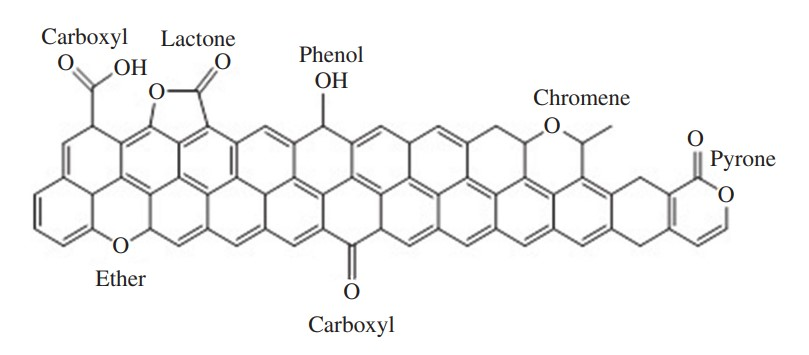
\includegraphics[width=0.8\linewidth]{surface functional group.jpg}
    \caption{Oxygen-containing surface functional group.}
    \label{fig:2.1.1.2}
\end{figure}

\vspace{0.3em}


\newpage
The oxygen-containing functional group is profoundly impacted by the pyrolysis temperatures. At low pyrolysis temperatures, the acidic functional groups are relatively abundant, making the produced biochars tend to be acidic, hydrophilic, and polar, whereas the biochars tend to be alkaline, hydrophobic, and nonpolar at higher pyrolysis temperatures, as the acidic functional groups are gradually eliminated and the concentratio of carbonat, ash, and inorganic alkali salts is higher \cite{Sajjadi2019} \cite{Tomczyk2020}. 

\vspace{0.3em}

In addition to oxygen-containing groups, biochars made from nitrogen-rich feedstocks like manure or sewage sludge may contain nitrogen-containing groups (such pyrrolic and pyridinic N), which provide additional Lewis base sites important for the adsorption of acidic contaminants.


%During pyrolysis, under increasing temperature, the higher degree of carbonization reduces the atomic ratios of H/C, O/C,and N/C, followed by a reduction in the abundances of carboxylic, hydroxyl, and amino groups.

%The O/C value represents the quantity of superficial polar functional groups and the hydrophilicity of BC, whereas the H/C value indicates the aromatization of the organic structure (Fang et  al. 2014, Han et  al. 2017). During pyrolysis, under increasing temperature, the higher degreeof carbonization reduces the atomic ratios of H/C, O/C, and N/C, followed by a reduction in the abundances of carboxylic, hydroxyl, and amino groups. Different elements of BC are (usually) determined by dry combustion, 




%whereas these elements respectively contribute to different functional groups that influence and determine other chemical properties, such as pH and nutrient value, as well as cation exchange capacity \cite{Munzeiwa2025BiocharBaselinePotential}. Oxygen contributes in forming surface functional groups, including hydroxyl and carboxyl that influence the pH value and cation exchange capacity of biochar. On the other hand, sulfur and phosporus content still associated with the pH value and CEC, while nitrogen content associated with the nutrient value \cite{Munzeiwa2025BiocharBaselinePotential}. 

%Oxygen content influences the resulting surface functionalities (e.g., hydroxyl, carboxyl, etc.) resulting in acidic biochar and improved cation exchange Content courtesy of Springer Nature, terms of use apply. Munzeiwa et al. Discover Water (2025) 5:77 Page 6 of 48 capacity (CEC). Biomass with higher oxygen content tends to have a lower carbon content but enhanced pore structure and surface area [69]. The elemental ratios C/H, C/O, and H/O can be used as indices for baseline potential, energy content, and environmental consequences of the biomass [160]. Whereas a higher C/H ratio predisposes biochar characterized by high aromaticity and stable graphic microstructure, a low C/H ratio indicates highly aliphatic biomass that is susceptible to decomposition [160]. A higher C/O ratio shows low oxygen content, resulting in more carbonization and lower reactivity [161].
%Nitrogen content influences the diversity of chemical moieties of the surface by contributing to the formation of functional groups such as amines, amides, pyrroles, pyridines, and nitriles, while sulfur contributes to thiols, sulfides, sulfonic acids, and sulfates, and P forms phosphates and phosphites which influence the pH and CECs of the resulting biochar [99, 100].

%\label{Properties of Biochar}
%\subsubsection*{pH}

%The pH of biochar is one the crucial chemical property in order to determine its application involving soil, since soil has varying levels of acidity and alkalinity. Acidic 


%Surface functional groups are an important chemical characteristic of biochar because they strongly influence its reactivity, interaction with water, nutrient retention, and adsorption behaviour. Although biochar is mainly described as a carbon-rich material, its surface is not chemically uniform. Instead, it contains different functional groups attached to the carbon matrix, particularly oxygen-containing groups such as hydroxyl, carboxyl, carbonyl, phenolic, lactone, ether, and quinone groups. Depending on the feedstock material and the production conditions, biochar may also contain nitrogen-, phosphorus-, or sulfur-containing functional groups, although these are usually present in smaller amounts compared with oxygen-based groups

\label{Properties of Biochar}
\subsubsection*{Specific Surface Area and Porosity}

The physical properties of biochar are primarily characterized by its specific surface area and porosity, which determine the reactivity and adsorption capacity of biochar \cite{Ingle2024}. Biochar displays high porosity with pores ranging from micro- (<2 nm) to macropores (>50 nm) \cite{Tomczyk2020} \cite{Sajjadi2019}, while the size of its specific surface area also vary. They are influenced by BC feedstock, pyrolysis temperature, and the activation process \cite{Sajjadi2019}. High pyrolysis temperature stimulates micropores formation, leading to larger specific surface area \cite{Sajjadi2019}. Micropores are also mainly formed from cellulose-enriched feedstock, whereas macropores are mainly observed in lignin-enriched feedstocks based biochar. The specific surface area and porosity of crop-residue-derived biochar are much bigger compared to those of animal-li-derived biochar, which is caused by the higher carbon content of plant-derived biochar \cite{Tomczyk2020} \cite{Sajjadi2019}. 

\begin{table}[H]
\centering
\caption{Specific surface area of different biochars. PT = pyrolysis temperature; SSA = specific surface area \cite{Tomczyk2020}.}
\label{tab:biochar_ssa_selected}

\small
\resizebox{0.75\textwidth}{!}{%
\begin{tabular}{l c c l}
\toprule
\textbf{Biomass feedstock} & \textbf{PT ($^\circ$C)} & \textbf{SSA (m$^2$/g)} & \textbf{Reference} \\
\midrule

Sugarcane bagasse & 400 & 0.8  & Ding et al. \cite{Ding2014BagasseBiochar} \\
Rapeseed plant    & 400 & 16.0 & Karaosmanoglu et al. \cite{Karaosmanoglu2000RapeseedCake} \\
Cow manure        & 400 & 2.5  & Kolodynska et al.\cite{Kolodynska2012BiocharMetalIons} \\
Pig manure        & 400 & 15.6 & Kolodynska et al.\cite{Kolodynska2012BiocharMetalIons} \\

\bottomrule
\end{tabular}%
}

\vspace{0.3em}
\end{table}

As example, figure~\ref{fig:bgr_biochar} illustrates the surface area and porosity of  plant-based charcoal and biochar. The charcoal and gasification coke produced from beech wood exhibit a porous surface structure, which is associated with a larger accessible surface area. By contrast, the flash-pyrolysis coke produced from spruce wood is covered by a resin layer, which reduces the accessible surface and limits the development or exposure of pores. 

\begin{figure}[ht!]
    \centering
    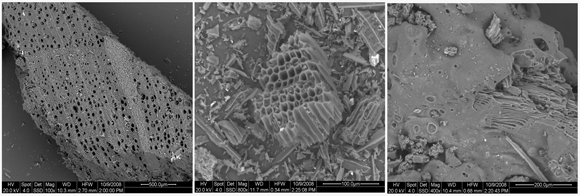
\includegraphics[width=1\textwidth]{Abbildungen/Biokohle.png}
    \caption{Surface area and porosity of charcoal from beech wood (left), gasification coke from beech wood (middle) and flash-pyrolisis coke from spruce wood (right)\cite{BGRBiochar}}
    \label{fig:bgr_biochar}
\end{figure}

\vspace{0.3em}

\subsubsection{Physical Activation of Biochar}

Physical activation refers to a method to produce activated biochar that has a larger surface area, wide range of functional groups and a more
uniform pore size distribution, leading to improvement on adsorption capacity of biochar. The most established and practically used physical approach is to activate the biochar by treating it with oxidizing agent, mainly steam and carbon dioxide, at temperature above 700°C. During this gaseous activation, oxidizing agents penetrate and gasify the structure of biochar consisting mainly from carbon atom, resulting in newly open and wider blocked pores. Therefore, activated biochar has higher internal surface areas and more oxygen functional groups as adsorption active sites \cite{sajjadi-2018}. 

\label{Physical Activation of Biochar}
\subsubsection*{Steam Activation}



Together with carbon dioxide 









%Steam activation is one of the oldest and most well-established methods for the physical activation of carbonaceous materials (Marsh and Reinoso, 2006). The process involves exposing biochar to superheated steam, typically at temperatures ranging from 700 to 900°C, for durations spanning from 30 minutes to several hours (Demiral et al., 2011; Girgis et al., 2011; Han et al., 2013). The smaller molecular size of water compared to CO₂ is a fundamental advantage of steam as an activating agent, as it facilitates deeper diffusion into the internal pore network of the biochar, inducing a faster and more thorough reaction throughout the material (Dalai and Azargohar, 2007). Unlike air activation, the reaction between steam and carbon is endothermic in nature, which makes it inherently more controllable and better suited for the activation of carbons with high surface activity (Sajjadi et al., 2018).
%The overall reaction mechanism of steam activation with biochar involves several sequential and concurrent steps, beginning with the chemisorption of water molecules onto active carbon surface sites (Lussier et al., 1998). In this initial step, oxygen from the water molecule is transferred to the carbon surface, forming a surface oxide complex while releasing hydrogen gas. This surface oxide may subsequently desorb from the carbon surface as carbon monoxide, regenerating an active carbon site. The carbon monoxide produced can further participate in the gasification process by scavenging additional surface oxide species to yield carbon dioxide. A water-gas shift reaction then proceeds in parallel, in which water vapor is decomposed into carbon dioxide and hydrogen gas (Sattar et al., 2014; Ferreira et al., 2017). The hydrogen produced can go on to further activate the carbon surface or inhibit gasification depending on local concentration. Hydrogen produced during these reactions has been shown to adsorb onto active carbon sites, forming stable surface hydrogen complexes that effectively block and deactivate those sites, thereby inhibiting further gasification (Lussier et al., 1998). Hydrogen adsorbed onto carbon surfaces requires temperatures as high as 1500°C for complete desorption, as detailed by Redmond and Walker (1960), meaning that the inhibitory effect of hydrogen is a persistent feature of the steam activation process that must be carefully managed through control of activation temperature and steam flow rate. Hüttinger (Hermann and Hüttinger, 1986) identified three possible mechanisms by which hydrogen inhibits steam gasification: dissociative hydrogen adsorption onto free active carbon sites, reverse oxygen exchange between hydrogen and surface oxides, and the scavenging of surface oxides by hydrogen gas.

\newpage
\label{Physical Activation of Biochar}
\subsubsection*{\textbf{CO$_2$} Activation}

The mechanism of biochar activation with carbon dioxide 






The mechanism of char (C) activation with CO2
involves the Boudouard reaction (C + CO2 ↔ 2CO). In this
process, CO2 undergoes dissociative chemisorption on the
carbon surface to form a surface oxide and carbon mon-
oxide as shown in R12. The surface oxide, C(O), is sub-
sequently desorbed from the surface, further developing
the pore structure (R13). CO in the gaseous product can
also be adsorbed on the carbon active site and retards the
gasification (R14).



\newpage
\subsubsection{Sulfur Loading of Biochar}

Sulfur loading refers to a process for increasing the sulfur content in biochar by exposing it to sulfur compounds, primarily hydrogen sulfide. The concept of sulfur loading is identical to the hydrogen sulfide removal process, which lets elemental sulfur to be adsorbed on the surface of biochar. In this process, the elemental sulfur is formed through the partial oxidation of hydrogen sulfide by oxygen in air \cite{Lin2025H2SOxidationPETBiochar}. Full oxidation is avoided to prevent the formation of unwanted sulfur dioxide ($SO$_2$) or sulfate ($SO$_4^{2-}$).

\begin{equation}
H_2S + \frac{1}{2}O_2 \rightarrow S + H_2O
\end{equation}

This process is favored for activated biochar due to its larger specific surface area and modifiable porosity compared to pristine biochar \cite{Lin2025H2SOxidationPETBiochar}. 

\vspace{0.3em}



%Sulfur loading of biochar refers to the enrichment of biochar with sulfur-containing species through adsorption, impregnation, or reaction with sulfur compounds. This modification is commonly applied to improve the chemical functionality of biochar and to expand its potential use as a soil amendment, fertiliser, or adsorbent material. In general, pristine biochar already contains a certain amount of sulfur depending on the original feedstock. However, the sulfur content is often relatively low compared with other major elements such as carbon, oxygen, potassium, calcium, and phosphorus. The total sulfur content of biochar is strongly influenced by feedstock type. 

%Sulfur loading can be carried out by exposing biochar to sulfur-containing gases, especially hydrogen sulfide (H$_2$S), or by treating it with sulfur-containing solutions. One important example is the use of activated biochar to remove H$_2$S from biogas streams. H$_2$S is a toxic and corrosive gas commonly produced during anaerobic digestion, and its removal is necessary to prevent equipment corrosion and environmental problems. Biochar can act as an adsorbent for H$_2$S due to its porous structure, surface area, pH, mineral content, and surface functional groups. In addition to physical adsorption, biochar can also promote the oxidation of H$_2$S into other sulfur forms, such as elemental sulfur and sulfate. These reactions are influenced by the surface chemistry of the biochar, including oxygen-containing functional groups, aromatic carbon structures, and catalytic elements such as iron and calcium.

%The effectiveness of sulfur loading depends strongly on the properties of the biochar. A higher surface area and well-developed pore structure can provide more adsorption sites for sulfur compounds. The pyrolysis temperature and activation process also play important roles because they influence the surface area, pore volume, pH, and the stability of functional groups. For example, steam activation can increase the surface area and microporosity of biochar, making it more suitable for gas adsorption. In the study by Zhang et al., sulfur-enriched biochar was produced by passing landfill biogas through a packed column containing activated biochar. The biochar used in this process was produced from anaerobically digested solid dairy manure and then steam activated. After exposure to H$_2$S-containing gas, the resulting sulfur-loaded biochar, referred to as SulfaChar, showed a sulfur content of 36.5%, compared with only 2.7% in the original biochar. This confirms that biochar can adsorb and retain a significant amount of sulfur from H$_2$S gas.

%Sulfur-loaded biochar is interesting not only as a gas-cleaning material but also as a potential fertiliser. Sulfur is an essential plant nutrient because it is involved in protein synthesis, enzyme activity, and chlorophyll formation. When sulfur is retained in biochar as plant-available forms such as sulfate, the material may function as a slow-release sulfur source in soil. Zhang et al. reported that SulfaChar increased corn biomass and enhanced the uptake of sulfur as well as other macro- and micronutrients, including nitrogen, phosphorus, potassium, calcium, magnesium, zinc, manganese, and boron. This suggests that sulfur-loaded biochar can act either as a direct nutrient supplier or as a carrier material that improves nutrient uptake efficiency.

%Biochar, enriched with sulfur, has recently emerged as a promising alternative in sustainable agricultural practices, particularly as a means of enhancing soil fertility. This approach addresses the dual challenge of managing environmental contamination and optimizing resource utilization. Conventional fertilizers, although effective in nutrient delivery, often pose risks to ecosystems due to their propensity for nutrient runoff and chemical leaching, contributing to ecological imbalance. Hence, biochar enriched with sulfur offers an eco-friendly and resource-efficient solution by improving nutrient retention capacity, promoting soil organic matter content, and subsequently enhancing plant productivity. On the other side, sulfur enrichment of biochar can be achieved through the adsorption of hydrogen sulfide ($H_2S$), a highly toxic and corrosive gaseous contaminant commonly produced during the anaerobic digestion of organic waste for methane generation. Recent studies indicate that biochar possesses substantial potential as an effective adsorbent for $H_2S$ removal from biogas, thereby not only mitigating the environmental hazards associated with $H_2S$ emissions but also creating a value-added sulfur-enriched biochar suitable for agricultural use. 

\subsubsection{Utilization of Biochar}

Biochar has broad application depending to its modifications. 

\newpage
\setresponsible{Surya Salim}
\subsection{Pyrolisis}

%https://www.intechopen.com/chapters/78772
%https://www.intechopen.com/books/10862
%https://www.mdpi.com/1996-1073/5/12/4952
\subsubsection{Definition and principle of pyrolysis}
Pyrolysis is one of the most widely used thermochemical methods for converting biomass and producing biochar. It involves the thermal decomposition of organic material under an inert atmosphere, in the absence of oxygen, yielding three primary products: char, bio-oil, and syngas. Bio-oil is a complex liquid mixture composed of hundreds of oxygenated compounds, which can be further upgraded using specialized catalysts to produce biofuels or value-added chemicals. During pyrolysis, the complex molecular structure of biomass is broken down into smaller, simpler components, resulting in the formation of both a vapor phase and a solid phase \cite{Dufour2016}.

\subsubsection{Slow versus Fast Pyrolysis}
Pyrolysis of biomass is broadly classified into three modes: slow, intermediate, and fast pyrolysis. The key parameters governing this classification, which also serve as the primary operating conditions, are the heating rate, temperature, and vapor residence time \cite{Vuppaladadiyam2022}.
\vspace{0.3em}
\newline
Fast pyrolysis is characterized by very high heating rates (typically exceeding 100 °C/s), short vapor residence times of less than 2 seconds, and moderate temperatures ranging from 500 to 700 °C. These conditions promote rapid thermal decomposition, favoring the production of liquid products — particularly bio-oil — which can reach yields of up to 70–75 wt.\% \cite{Lehmann2015,Luque2016}.
\vspace{0.3em}
\newline
In contrast, slow pyrolysis operates at lower heating rates (0.1–1 °C/s), longer residence times (minutes to hours), and temperatures typically ranging from 300 to 700 °C. Under these conditions, volatile compounds remain in contact with the solid phase for longer periods, enabling secondary reactions that promote char formation. This mode of pyrolysis is preferred when the primary objective is to maximize biochar yield, a process also referred to as carbonization \cite{Lehmann2015,Pahnila2023}.
As a result of these process differences, slow pyrolysis is primarily employed for biochar production, whereas fast pyrolysis is optimized for bio-oil production. The prolonged interaction between vapors and the solid phase in slow pyrolysis enhances carbonization, leading to higher solid yields. Consequently, slow pyrolysis is the preferred thermochemical conversion route when the objective is to produce stable, carbon-rich biochar with well-developed structural properties.

\begin{table}[H]
\centering
\caption{Comparison of slow and fast pyrolysis for biomass (adapted from \textcite{Tan2021})}
\label{tab:pyrolysis_comparison}
\small
\begin{tabular}{p{2.5cm} p{6cm} p{6cm}}
\hline
\textbf{Features} & \textbf{Slow Pyrolysis} & \textbf{Fast Pyrolysis} \\
\hline
Temperature (°C) & 300–700 & 600–1000 \\[3pt]
Heating rates (°Cmin$^{-1}$) & 0.1–10 & 10–10000 \\[3pt]
Aeration & Oxygen-free or limited & Oxygen-free \\[3pt]
Residence Time & Minutes–hours & Seconds \\[3pt]
Target product & Biochar & Bio-oil \\[3pt]
Advantages & -The highest yield of biochar. \newline -Can accept a wide range of particle size. & -A higher yield of bio-oil. \\[3pt]
Disadvantages & Further treatment of gases is needed due to high CO concentrations & -Low biochar yield. \newline -Fine particle of biomass feed (1–2mm) is required. \newline -Prefer biomass with low moisture content ($<$10\%) \\[3pt]
\hline
\end{tabular}
\end{table}


\subsubsection{Thermal decomposition of biomass components}
Biomass subjected to pyrolysis typically consists of a mixture of organic and inorganic constituents, including lignocellulosic components (cellulose, hemicellulose, and lignin), as well as proteins, lipids, and mineral matter. The thermal decomposition behavior of these constituents plays a crucial role in determining the yield and properties of the resulting biochar \cite{Yang2007,Wen2021}.

\vspace{0.3em}

The lignocellulosic fraction exhibits distinct thermal decomposition characteristics. Hemicellulose is the least thermally stable component, decomposing at relatively low temperatures, typically between 150 °C and 300 °C. Cellulose decomposes at slightly higher temperatures, generally in the range of 320 °C to 400 °C, and is characterized by a sharp and narrow degradation profile. In contrast, lignin decomposes over a much broader temperature range, from approximately 250 °C up to 600 °C or higher, owing to its complex aromatic structure \cite{ElSayed2023,Chen2026}.

\vspace{0.3em}

The overall pyrolysis process can be divided into several stages. At temperatures below approximately 220 °C, moisture evaporation dominates. Between 220 °C and 400 °C, rapid devolatilization occurs, primarily due to the decomposition of hemicellulose and cellulose. At higher temperatures, above 400 °C, lignin degradation and carbonization become dominant, leading to the formation of a carbon-rich solid residue \cite{Yang2005,ElSayed2023}. Notably, compared to cellulose and hemicellulose, lignin decomposes more slowly and contributes significantly to char formation owing to its high thermal stability and complex aromatic structure. Consequently, lignin is considered the primary precursor for biochar formation during pyrolysis \cite{Chen2022}.

\vspace{0.3em}

In addition to lignocellulosic components, digestate-based feedstocks contain proteins, lipids, and inorganic minerals, which further influence pyrolysis behavior. Proteins decompose to form nitrogen-containing compounds, that affect the nitrogen content of the resulting biochar\cite{Navarro2025}. Lipids tend to promote the formation of liquid products, while inorganic minerals can act as catalysts, altering reaction pathways and influencing pore development. Furthermore, interactions between these components during pyrolysis can lead to non-additive effects, resulting in complex product distributions and structural characteristics of biochar \cite{Puri2024,Kebelmann2013}.

\begin{table}[H]
\centering
\caption{Biomass components and their role during pyrolysis\cite{Chen2022,Armanu2024,Puri2024}}
\label{tab:biomass_components}
\small
\begin{tabular}{p{2cm} p{2.2cm} p{1.8cm} p{3.2cm} p{2.5cm} p{3cm}}
\hline
\textbf{Component} & \textbf{Typical Decomposition Temperature} & \textbf{Thermal Stability} & \textbf{Main Role During Pyrolysis} & \textbf{Effect on Char Formation} & \textbf{Key Notes} \\
\hline
Hemicellulose & $\sim$150–300°C & Low & Decomposes early $\rightarrow$ releases CO$_2$, volatiles & Very low & Produces mostly gases and light compounds; little solid residue \\[6pt]

Cellulose & $\sim$320–400°C & Medium & Rapid depolymerization $\rightarrow$ volatiles (e.g. levoglucosan) & Moderate & Can contribute to char under certain conditions\cite{Armanu2024} \\[6pt]

Lignin & $\sim$250–600°C (wide range) & High & Slow decomposition $\rightarrow$ aromatic structures & High (dominant) & Main precursor for stable biochar \\[6pt]

Proteins & $\sim$200–500°C & Medium & Decompose $\rightarrow$ NH$_3$, N-compounds & Indirect & Increase nitrogen content in biochar \\[6pt]

Lipids (fats) & $\sim$300–500°C & Medium & Crack into hydrocarbons and oils & Low / negative & Promote bio-oil formation $\rightarrow$ reduce char yield \\[6pt]

Mineral matter (ash) & Non-decomposing (inorganic) & Very high & Catalyzes reactions & Indirect (can increase or decrease) & Alters decomposition pathways and pore structure \\
\hline
\end{tabular}
\end{table}

\subsubsection{Influence of Pyrolysis Condition on Bichar Properties}
\label{Influence pyrolysis condition}
\subsubsection*{Effect of Temperature on Biochar}
\label{subsubsec:Effect of Temperature on Biochar}
Pyrolysis temperature is one of the most influential parameters governing the physicochemical properties of biochar. It directly affects the extent of thermal decomposition, carbonization, and structural transformation of biomass, thereby determining the resulting biochar yield, elemental composition, porosity, and stability \cite{Lataf2022}.

\vspace{0.3em}

With increasing pyrolysis temperature, biochar yield generally decreases due to the enhanced release of volatile compounds, such as gasses and condensable vapors. At lower temperatures, incomplete decomposition leads to higher retention of solid mass, whereas higher temperatures promote devolatilization and reduce the remaining char fraction \cite{zhang-2014}.

\vspace{0.3em}

Simultaneously, increasing pyrolysis temperature leads to a higher degree of carbonization, reflected in a rising carbon content and a concurrent decrease in hydrogen and oxygen content, resulting in a more aromatic and condensed carbon structure. Consequently, biochar produced at higher temperatures exhibits enhanced thermal stability and resistance to degradation \cite{zhang-2014,zhang-2022,224pyrolysistemp}.

\vspace{0.3em}

In addition, elevated pyrolysis temperatures promote the development of pore structures due to the progressive release of volatile matter. This results in increased surface area and porosity, which are important for adsorption-related applications. However, excessively high temperatures may also lead to pore widening or structural collapse, depending on the feedstock and process conditions \cite{tomczyk-2020,ghorbani-2022}.

\vspace{0.3em}

Overall, pyrolysis temperature governs a fundamental trade-off between biochar yield and quality: lower temperatures favor higher yields but produce less stable and less carbonized materials, while higher temperatures enhance structural stability, carbon content, and porosity at the expense of reduced yield.


\subsubsection*{Effect of Heating Rate on Biochar}

Heating rate is one of the operational parameters that must be defined in pyrolysis. It influences thermal decomposition pathways, volatile release, and the physicochemical properties of the resulting biochar. As a general rule of thumb, slow heating rates promote gradual devolatilization and prolong the interaction between volatile compounds and the solid phase, thereby favoring secondary charring reactions and enhancing solid carbon formation \cite{awad-2024,brunner-1980}.

\vspace{0.3em}

Compared to rapid heating conditions, low heating rates are commonly associated with higher char yields and improved structural ordering of biochar. Slow pyrolysis conducted at heating rates in the range of approximately 10–30 °C/min has been widely reported as suitable for maximizing biochar production \cite{awad-2024}.

\vspace{0.3em}

In addition, heating rate can influence pore development and carbon structure formation. Previous studies have shown that slowly carbonized biomass may exhibit larger micropore volumes and more developed surface characteristics compared to rapidly heated samples \cite{awad-2024,song-2025}.
In the present study, a constant heating rate of 10 °C/min was selected to ensure controlled thermal decomposition under slow pyrolysis conditions and to promote the formation of stable, carbon-rich biochar.


\subsubsection*{Effect of Residence Time on Biochar}
Residence time is another important operational parameter in pyrolysis, as it influences the extent of devolatilization, carbonization, and structural transformation of biomass during thermal decomposition. Longer residence times allow biomass to remain at elevated temperatures for extended periods, thereby promoting further decomposition of volatile compounds and the formation of more condensed carbon structures \cite{leng-2018,wang-2019}. Several studies have reported that increasing residence time can reduce biochar yield due to the continued release of volatile matter and secondary cracking reactions. At the same time, extended residence times are generally associated with higher pH values, increased ash content, and greater aromaticity of the resulting biochar \cite{sun-2016,wijitkosum-2023}.

\vspace{0.3em}

Residence time also affects the physicochemical structure of biochar, including surface area and pore development. Moderate residence times may enhance pore formation and surface characteristics, whereas excessively long residence times can lead to pore widening or partial structural collapse \cite{wang-2019}. However, compared to pyrolysis temperature, the influence of residence time on biochar properties is often less pronounced. Previous studies have reported that pyrolysis temperature is generally the dominant parameter governing biochar characteristics, while the effects of residence time are comparatively minor \cite{wang-2020, zhao-2017}.

\vspace{0.3em}

In the present study, a constant residence time of 1 hour was selected to ensure sufficient devolatilization and stable carbonization under slow pyrolysis conditions. Although pyrolysis temperature was the principal variable investigated, the selected heating rate and residence time also contributed to the final physicochemical properties of the produced biochars.

\vspace{0.3em}

The physicochemical properties of biochar are strongly governed by pyrolysis conditions such as temperature, heating rate, and residence time. These process parameters directly influence the elemental composition, aromaticity, pore structure, surface functionality, and stability of the resulting biochar, thereby determining its suitability for specific applications \cite{luo-2024,tomczyk-2020}.
For soil amendment applications, biochar produced at relatively lower pyrolysis temperatures generally retains a higher proportion of oxygen-containing functional groups and volatile matter, which may enhance nutrient exchange capacity and microbial interactions in soil. In contrast, biochar produced at higher temperatures typically exhibits greater aromaticity, higher carbon stability, and increased resistance to microbial degradation, making it more suitable for long-term carbon sequestration and persistent soil conditioning \cite{lu-2021,nogues-2023,pokharel-2025}.
Pyrolysis temperature also significantly influences pore development and surface area. Elevated temperatures promote devolatilization and the formation of more developed porous structures, which are beneficial for adsorption-related applications such as wastewater treatment, gas purification, and contaminant removal. Higher-temperature biochars generally possess larger surface areas and improved adsorption performance due to increased aromaticity and pore formation \cite{loebsack-2025,luo-2024}.
In addition, biochar characteristics relevant to soil improvement — including water-holding capacity, cation exchange capacity, pH, and microbial interactions — are strongly dependent on pyrolysis conditions. Several studies have reported that biochar produced within intermediate-to-high temperature ranges may significantly improve soil aggregation, water retention, and long-term soil carbon conservation \cite{ghorbani-2022,kabir-2023,shyam-2025}.
Therefore, optimization of pyrolysis conditions is essential to tailor biochar properties for targeted applications. Lower-temperature biochars may be more favorable for nutrient-related and biologically active soil applications, whereas higher-temperature biochars are generally preferred for adsorption processes, contaminant remediation, and long-term carbon sequestration.

\subsubsection{Relevance of Pyrolysis for digestate-derived biochar}
\label{subsubsec:digestate-pyrolysis relevance}
Digestate-derived biochar differs significantly from biochar produced from conventional lignocellulosic biomass such as wood, straw, or agricultural residues. Digestates represent complex biomass matrices containing partially degraded organic matter resulting from anaerobic digestion, as well as elevated mineral and ash contents. In addition to residual lignocellulosic structures, digestates may contain proteins, lipids, and inorganic compounds, all of which influence thermal decomposition behaviour during pyrolysis \cite{kujawska-2026,sarkar-2024}.

\vspace{0.3em}

Due to this heterogeneous composition, the physicochemical properties of digestate-based biochar are strongly dependent on pyrolysis temperature. Pyrolysis temperature governs the extent of devolatilization, carbonization, aromatization, and pore development, thereby determining the resulting yield, elemental composition, stability, and surface characteristics of biochar \cite{kujawska-2026, manya-2012}.

\vspace{0.3em}

At relatively low pyrolysis temperatures of around 400 °C, carbonization remains incomplete and the resulting biochar typically retains a larger proportion of volatile matter and oxygen-containing functional groups. Consequently, low-temperature biochars often exhibit higher yields, greater chemical reactivity, and improved nutrient exchange capacity. However, their carbon structure is generally less aromatic and less resistant to microbial degradation \cite{wystalska-2021}.

\vspace{0.3em}

Intermediate pyrolysis temperatures of around 500 °C are commonly regarded as a transition region between incomplete carbonization and the formation of more condensed aromatic carbon structures. Within this temperature range, biochar may exhibit a balance between yield retention and improved physicochemical properties, such as thermal stability and pore development \cite{alghashm-2023,kujawska-2026}.

\vspace{0.3em}

At higher pyrolysis temperatures of around 600 °C, devolatilization and carbonization become more pronounced, resulting in biochar with increased aromaticity, enhanced thermal stability, and more developed pore structures. Elevated temperatures also promote the elimination of hydrogen- and oxygen-containing functional groups, leading to more carbon-rich and chemically stable biochar materials \cite{kujawska-2026,wystalska-2021}.

\vspace{0.3em}

Several studies have reported that increasing pyrolysis temperature generally reduces biochar yield due to the enhanced release of volatile compounds. However, digestate-derived biochars may exhibit more complex behavior owing to their elevated mineral and ash contents. Inorganic components such as potassium, calcium, magnesium, and phosphorus may catalytically influence pyrolysis reactions and alter char formation pathways, resulting in deviations from conventional lignocellulosic biomass trends\cite{kujawska-2026,wang-2023}.

\vspace{0.3em}

In the present study, pyrolysis temperatures of 400 °C, 500 °C, and 600 °C were selected to investigate the transition from partially carbonized digestate-derived biochar toward more thermally stable and aromatic carbon structures. Particular attention was given to the relationship between pyrolysis temperature and biochar yield, elemental composition, and surface morphology.


\newpage
\subsection{Calorific Value (HHV and LHV)}

\subsubsection*{Definition}
The two principal calorific descriptors of a solid fuel are the \textbf{higher heating value} (HHV; also termed Brennwert, gross calorific value, GCV, or $H_0$) and the \textbf{lower heating value} (LHV; also termed Heizwert, net calorific value, NCV, or $H_u$).
\begin{itemize}
    \item \textbf{HHV (Brennwert /  $H_0$ / GCV )} is defined as the absolute value of the specific energy of combustion, in joules, of unit mass of a fuel burned in oxygen in a calorimetric bomb under specified standard conditions, with the resulting water of combustion fully condensed to the liquid state at the reference temperature of 25°C \cite{iso18125_2017,din51900_2023,astm_d5865_2019}. HHV is therefore measured at constant volume.
    \item \textbf{LHV (Heizwert / $H_u$ / NCV)} is the corresponding heat of combustion calculated under conditions where the water of combustion remains in the vapor state. LHV at constant pressure is the operative quantity used in practical fuel applications (boilers, gasifiers, combustors), since flue gases generally leave the system above the dew point \cite{iso18125_2017, din51900_old,van-loo-2008}
\end{itemize}

The fundamental difference between HHV and LHV is therefore the inclusion (HHV) or exclusion (LHV) of the latent heat of vaporization ($\approx$ 2.442-2.453 MJ kg$^{-1}$ at 25 °C) of the water that is chemically formed by the combustion of the fuel-bound hydrogen and originally present in the fuel as moisture \cite{basu-2018,channiwala-2002}.

\subsubsection*{Why the Distinction Matters for Biomass and Biochar}
Biomass and digestate-derived chars typically contain non-trivial amounts of hydrogen (1-6 wt\% in chars, up to 6-7 wt\% in raw biomass) and moisture (5-60 wt\% as received). Because the latent heat term is mass-specific to the $H_2O$ formed/contained, neglecting the HHV→LHV correction can lead to errors of 1-3 MJ kg$^{-1}$ for biomass - i.e., 5–15\% of the energy content \cite{van-loo-2008,vargas-moreno-2012}. In biochars from high-ash, high-mineral feedstocks (such as slaughterhouse digestate), where HHV may already be modest (10-22 MJ kg$^{-1}$), reporting LHV vs HHV consistently is essential for honest energy balances and for downstream techno-economic assessments of pyrolysis-and-activation systems \cite{Lehmann2015}.

\subsubsection*{Conversion Formulae HHV $\leftrightarrow$ LHV}
The most widely used conversion at constant pressure, applicable to both biomass and biochar, is given in ISO 18125:2017 \cite{iso18125_2017} and reproduced in essentially identical form by virtually all biofuel handbooks \cite{van-loo-2008,basu-2018}:
\[
LHV_{p,ar} = HHV_d \times (1 - M/100) - 2.442 \times (M/100) - 2.442 \times 8.94 \times (H_d/100) \times (1 - M/100)        [MJ kg^{-1}]
\]

where $HHV_d$ is the gross calorific value on a dry basis (MJ kg$^{-1}$), $H_d$ the hydrogen content on a dry basis (wt\%), and M the moisture content as received (wt\%). The LHV$_{p,ar}$ itself represents the lower heating value, at constant pressure, on an as-received basis. The constant 2.442 MJ kg$^{-1}$ is the latent heat of vaporization of water at 25 °C, and the factor 8.94 = $M_{H2O}$/$M_{H2}$ = 18.015/2.016 converts hydrogen mass to the mass of water formed.
Equivalent simplified form often quoted in the literature \cite{sheng-2005}:
\[
LHV = HHV - 2.442 \times (9 H/100 + M/100) \qquad [MJ\, kg^{-1},\:H\: and\: M\: in\: wt\%]
\]

For dry-basis comparisons (M = 0), this reduces to 
\[
LHV_d = HHV_d - 0.21978 \times H_d \qquad [MJ kg^{-1},\: H_d\: in\: wt\% ]
\]

\subsubsection{Relevance of calorific Value for Biomasss, Digestate and Biochar}
HHV and LHV are universally regarded as the single most important physico-chemical properties for evaluating solid fuels, because they directly govern the thermal output per unit mass that can be released by combustion and thus the techno-economic viability of any thermal-utilization pathway \cite{van-loo-2008,basu-2018,Lehmann2015}. They are also a required input for energy balances of pyrolysis processes (energy yield, energy densification factor) and for the classification of solid biofuels under EN ISO 17225 and the European Biochar Certificate (EBC) standard.

\subsubsection*{Typical HHV Ranges}
\begin{table}[H]
\centering
\caption{Typical higher heating values (HHV) of various fuel categories}
\label{tab:hhv_fuels}
\small
\begin{tabular}{p{3.5cm} p{4cm} p{4.5cm}}
\hline
\textbf{Fuel category} & \textbf{HHV (MJ kg$^{-1}$, dry basis)} & \textbf{Reference} \\
\hline
Lignocellulosic biomass (wood, straw) & 17--19 & \textcite{van-loo-2008} \\[6pt]
Herbaceous / agricultural residues & 15--18 & \textcite{vassilev-2009} \\[6pt]
Raw digestate (anaerobic) & 14--17 (often lower because of high ash) & \textcite{neumann-2014}; \textcite{pecchi-2019} \\[6pt]
Lignocellulosic biochar & 25--33 & \textcite{Lehmann2015} \\[6pt]
Charcoal from wood & 30--34 & \textcite{antal-2003} \\[6pt]
Bituminous coal & 28--33 & \textcite{channiwala-2002} \\
\hline
\end{tabular}
\end{table}

Specific representative values:
\begin{itemize}
    \item Solid digestate (biogas plant, food/agricultural origin): HHV $\approx$ 15.0 - 17.1 MJ kg$^{-1}$ (\textcite{neumann-2014}).
    
    \item Solid digestate with high ash ($\approx$ 23 wt\% ash): HHV $\approx$ 16.6 MJ kg$^{-1}$ (\textcite{hung-2017}).
    
    \item Slaughterhouse meat-and-bone meal (MBM): HHV $\approx$ 13 - 30 MJ kg$^{-1}$ (\textcite{cascarosa-2011}).
\end{itemize}

\subsubsection*{Energy Densification Factor}
The energy densification ratio (or energy densification factor, EDF) is defined as
\begin{equation}
    EDF = HHV_{biochar} / HHV_{feedstock}  
\end{equation}
             
and the energy yield, considered in conjunction with mass yield, as
\begin{equation}
    Y_E = (m_{biochar} / m_{feedstock}) \times (HHV_{biochar} / HHV_{feedstock})  
\end{equation}
\cite{bridgwater-2011,antal-2003}. For lignocellulosic feedstocks pyrolysed at 400 - 600°C, EDF is typically 1.4 - 1.8 with energy yields of 50–75 \%; for high-ash digestates, EDF is generally lower than 1.4 and may be $\leq$ 1, because ash dilution can outweigh organic carbon enrichment \cite{hung-2017, opatokun-2015}.

\subsubsection{Effect of Pyrolysis Temperature on Calorific Value of (Digestate-Derived) Biochar}


\subsubsection*{General Trend for Lignocellulosic Biochar}
For wood and herbaceous feedstocks, increasing pyrolysis temperature from ~300 °C to 600 - 700 °C consistently elevates HHV. Carbon content typically rises from 50 - 55 wt\% (raw biomass) to 75–90 wt\% in 600 °C biochar, while H/C and O/C atomic ratios drop sharply, indicating progressive aromatization and dehydration/decarboxylation \cite{tag-2016,babu-2024}.

\subsubsection*{Trend for Digestate-Derived Biochar}
For digestate-based biochars the picture is qualitatively different and is critical for the present thesis. The dominant trend reported across multiple studies is that HHV plateaus, levels off, or even decreases with rising pyrolysis temperature. This was driven primarily by progressive ash concentration, which preserves the inorganic fraction while combustible volatiles are released. Calcination and shrinkage of mineral phases at higher temperatures further suppress the calorific value \cite{hung-2017, pecchi-2019}.

\vspace{0.3em}

Reported HHV values for digestate-derived biochars typically fall in the range of 13-22 MJ kg$^{-1}$, depending on feedstock origin and pyrolysis temperature:
\begin{table}[H]
\centering
\caption{HHV trends of digestate-derived biochar across pyrolysis temperature ranges}
\label{tab:hhv_digestate_comparison}
\small
\begin{tabular}{p{3.5cm} p{2cm} p{6cm} p{3cm}}
\hline
\textbf{Feedstock} & \textbf{T range (°C)} & \textbf{HHV trend} & \textbf{Reference} \\
\hline
Biogas digestate (food waste, 23 wt\% ash) & 300--900 & Decreasing from 16.6 MJ kg$^{-1}$ (raw) & \textcite{hung-2017} \\[6pt]
Food-waste digestate & 350--600 & 18.5 $\rightarrow$ 13--16 MJ kg$^{-1}$ & \textcite{opatokun-2015} \\[6pt]
Agricultural digestate & 300--700 & Capped at modest gains; ash rose 20 $\rightarrow$ $>$40 wt\% & \textcite{pecchi-2019} \\[6pt]
Agricultural biogas digestate & 400--600 & 17 $\rightarrow$ 19--22 MJ kg$^{-1}$ (peak at 400--500°C, then decline) & \textcite{kujawska-2026} \\[6pt]
OFMSW digestate & 300--700 & Ash rises monotonically, limiting HHV & \textcite{alghashm-2023} \\
\hline
\end{tabular}
\end{table}

\subsubsection*{Competing mechanisms}
The temperature dependence of biochar HHV is governed by two opposing effects:
\begin{enumerate}
    \item \textbf{Carbon enrichment / Aromatization} Raises HHV: As temperature increases, hydrogen- and oxygen-containing functional groups (-OH, -COOH, C=O) are progressively eliminated through dehydration, decarboxylation and condensation reactions, raising the C content and the degree of aromaticity. This per se increases the HHV on a daf basis.
    \item \textbf{Devolatilization and ash concentration} (lowers HHV on a whole-mass basis): The release of combustible volatile matter reduces solid mass while inorganic ash is retained, so the fraction of ash in the residual solid grows monotonically. For high-ash feedstocks, this dilution dominates \cite{alghashm-2023}.
\end{enumerate}
The net effect depends on the ash/organic ratio of the feedstock. For lignocellulosic biomass (ash 1-5 wt\%), effect (1) dominates and HHV rises with temperature. For digestate (ash 15–50 wt\%), effect (2) often overwhelms effect (1), and HHV can plateau or decline above ~500 °C \cite{Lehmann2015,antal-2003}.

\subsubsection*{Why Digestate-Derived Biochar Has Lower HHV than Wood-Derived Biochar}
There are some reasons that explain why biochar produced from digestate consistently exhibits a lower calorific value than its wood-derived counterpart, even when pyrolysed under same conditions.

\vspace{0.3em}

\textbf{First, the high mineral content of digestate fundamentally limits its energy density.}\newline
Anaerobic digestion concentrates inorganic elements - primarily Ca, P, K, Mg, and Si - in the solid residue, since these are not consumed by methanogenic microorganisms \cite{moller-2012,tambone-2010}. Because ash is non-combustible, it acts as a thermal diluent: every unit of ash mass displaces an equivalent mass of carbonaceous material that could otherwise contribute to combustion enthalpy. This effect is quantified directly in the \textcite{channiwala-2002} correlation, where ash carries a negative coefficient of –0.0211 MJ kg$^{-1}$ per wt\%.

\vspace{0.3em}

\textbf{Second, anaerobic digestion alters the organic composition of the residual solid in ways that reduce its fuel quality.} \newline
Methanogenic bacteria preferentially degrade easily hydrolysable carbohydrates - cellulose and hemicellulose - while lignin remains largely recalcitrant, which means that that the microorganisms in the biogas reactor struggle tyo break it down, so it largely passes through the digestion process intact and ends up concentrated in the digestate \cite{triolo-2011,monch-tegeder-2013}. The resulting digestate is therefore enriched in lignin, protein, and mineral matter relative to the original feedstock. While lignin itself has a relatively high HHV, the combined dilution by ash and moisture in the digestate matrix yields a substantially lower overall calorific value than "fully" lignocellulosic biomass \cite{pecchi-2019}.

\vspace{0.3em}

\textbf{Third, slaughterhouse digestate exhibits a particularly distinctive composition.} It typically contains paunch content, blood, fat residues, bone fragments, and proteinaceous matter \cite{salminen-2002,ware-2016}, which combine to give a unique profile: increased ash from bone-derived Ca-P phases, high nitrogen content from proteins, and significant moisture. Its calorific value is therefore comparable to meat-and-bone meal (MBM), with reported raw HHV values in the range of 13-30 MJ kg$^{-1}$ \cite{cascarosa-2011,conesa-2003,zaharioiu-2022}. After pyrolysis, biochar HHV typically falls within 15 - 22 MJ kg$^{-1}$, depending on temperature \cite{pecchi-2019,kujawska-2026}.

\subsubsection{Note on Steam (\texorpdfstring{H$_2$O}{H2O}) Activation}
Physical steam activation, applied after pyrolysis typically at temperatures above 700 °C and commonly around 800–900 °C, develops porosity by gasifying carbon through steam–carbon reactions such as $C$ + $H_2O$ → $CO$ + $H_2$. This process consumes part of the carbon matrix and can reduce the total solid mass or energy yield, although the HHV per unit mass may remain relatively stable depending on the feedstock and activation severity \cite{sajjadi-2018};
however, a study reports that steam-activated carbons produced from mixed conifer mill-residue biochars retained high higher heating values, ranging from approximately 27.7 to 31.1 MJ kg$^{-1}$. This indicates that activation did not eliminate the material’s energy content, although the study mainly evaluates the products as activated carbon/sorbents rather than as fuels \cite{anderson-2021}.





            




\subsubsection{Caloric Value Determination : Principle of Bomb Calorimetry}
\label{subsubsec:HHV}
Caloric value is determined by burning a precisely weighed sample in pure oxygen at an initial pressure of certain bar within a sealed, thermally insulated stainless-steel pressure vessel ("bomb"). It then immersed itself in a defined mass of water inside an insulated jacket. Combustion is initiated electrically via an ignition wire, and the heat released raises the temperature of the calorimeter-water system. The corrected temperature rise $\Delta T$ is converted into the gross calorific value using the calorimeter heat capacity C, previously determined by combustion of certified benzoic acid \cite{iso18125_2017,astm_d5865_2019}.

The general working equation is:
\begin{equation} \label{equ: qvgr}
    q_{V,gr}=(\varepsilon \cdot \Delta T - Q_{EXT} )/m
\end{equation}

where:
\begin{itemize}
    \item $q_{V,gr}$ = gross calorific value at constant volume (J $g^{-1}$);
    \item $\varepsilon$ = effective heat capacity of the calorimeter system (J K$^{-1}$), determined by calibration with benzoic acid (HHV = 26.434 kJ g$^{-1}$ at the certified reference state);
    \item $\Delta T$ = corrected temperature rise (K), corrected for heat exchange with surroundings (Regnault-Pfaundler or equivalent in static/isoperibolic mode; not required in adiabatic mode);
    \item $Q_{\mathrm{ext}}$ = sum of external corrections (ignition wire combustion, cotton thread, formation of HNO$_3$ from N$_2$ and H$_2$O, formation of H$_2$SO$_4$ from fuel-bound S);
    \item $m$ = sample mass (g).
\end{itemize}


\subsection{Scanning Electron Microscopy (SEM) analysis}
